\chapter{Introducción}
\label{ch:introducción}

Cualquier capítulo puede tener múltiples apartados, como el \autoref{sec:lista_de_items} o el \autoref{sec:enumeraciones} de este mismo capítulo.

También está el \autoref{sec:primera_sección} del \autoref{ch:capítulo-dos} que tiene la \autoref{fig:otra}.

Se puede utilizar \verb|\indent| o \verb|\noindent| al principio de un párrafo para añadir o eliminar la sangría en el párrafo, respectivamente.

\section{Listas de elementos}
\label{sec:lista_de_items}

Esta es la lista de elementos del \autoref{sec:lista_de_items}:

\begin{itemize}
    \item Item 1
    \begin{itemize}
        \item Item 1
        \item Item 2
        \item Item 3
        \item Item 4
    \end{itemize}
    
    \item Item 2
    \item Item 3
    \item Item 4
\end{itemize}

\section{Enumeraciones}
\label{sec:enumeraciones}

Esto es una lista enumerada, que puede estar relacionada con la \autoref{fig:introducción}:

\begin{enumerate}
    \item Item 1
    \begin{enumerate}
        \item Item 1
        \item Item 2
        \item Item 3
    \end{enumerate}
    \item Item 2
    \item Item 3
\end{enumerate}

\section{Figuras y tablas}

En la \autoref{fig:introducción} se puede ver una figura de ejemplo. Las tablas, las figuras y los algoritmos (ver el \autoref{sec:algoritmo-zzz}) son flotantes. Esto quiere decir que \LaTeX{} los intentará ubicar en el mejor lugar posible al componer el documento, intentando respetar ciertas reglas tipográficas. Como este lugar puede ser diferente a la posición que realmente ocupan en el texto, \textbf{es importante referenciar en el texto todas las figuras y las tablas}, en los diferentes puntos donde se hable de ellas.

\begin{figure}[htbp]
   \centering
   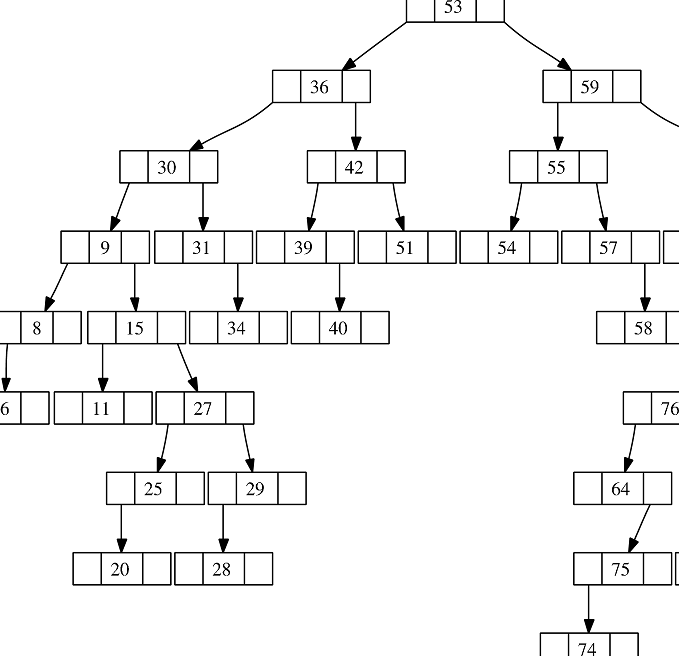
\includegraphics[width=0.8\linewidth]{images/figura_1}
   \caption{Ejemplo de figura.}
   \label{fig:introducción}
\end{figure}

La \autoref{tbl:presupuesto} en el \autoref{ch:presupuesto} es un ejemplo de tabla hecha con el paquete \verb|tabularx|.

Al crear tablas, figuras u otros elementos flotantes es aconsejable indicar siempre los especificadores de ubicación \verb|[htbp]|, tal y como se hace en los ejemplos de esta plantilla. De esta forma \LaTeX{} intentará primero ponerlos en el lugar; si no puede, intentará ponerlos en la parte superior o inferior de la misma página y, en caso extremo, los pondrá en páginas especiales que solo contienen flotantes.

No es buena idea usar especificadores como \verb|[!h]| o \verb|[H]| para forzar una ubicación determinada. El motivo es que eso impide a \LaTeX{} buscar la mejor forma de componer el documento, pudiendo dar como resultado páginas que se ven muy raras --por ejemplo, dejando muchos huecos libres entre el texto--.
Solo se deben utilizar estos especificadores cuando es absolutamente necesario, como ocurre en el \autoref{ch:presupuesto}, donde interesa que las tablas del presupuesto aparezca juntas, en la posición preestablecida.

\section{Código y algoritmos}

En el \autoref{ch:apéndice-uno} se pueden observar varios ejemplos de entornos para describir algoritmos y código.

\section{Citas}

Las referencias bibliográficas se deben indicar en el archivo \texttt{referencias.bib}, en formato Biblatex \cite{overleaf_biblatex}, y se citan en el texto. Las referencias no citadas no aparecerán en el apartado de la bibliografía.

Las citas pueden ser \emph{en línea} con el texto, como en \cite{examplegithub}, o entre paréntesis \parencite{examplearticle}. Sin embargo, no hay diferencia entre ambos tipos cuando se usa el estilo de cita numérico, que es el estilo por defecto en esta plantilla. Para apreciar la diferencia es necesario activar un estilo de cita como APA.

Las reglas para citar descritas en la guía de la ULL \cite{ulllibguide} permiten citar cualquier cosa: artículos de investigación, libros, entradas de la Wikipedia, blogs, vídeos de Youtube o repositorios de GitHub, entre otros. 

En el \autoref{ch:capítulo-cuatro} se puede ver otro tipo de cita, usando el paquete \texttt{csquotes}, donde se traslada de forma literal una porción del texto original al documento.
 
\section{Otra sección...}

\lipsum[1]

\subsection{Con subsección...}

\lipsum[2]